%iffalse
\let\negmedspace\undefined
\let\negthickspace\undefined
\documentclass[journal,onecolumn]{IEEEtran}
\usepackage{cite}
\usepackage{amsmath,amssymb,amsfonts,amsthm}
\usepackage{algorithmic}
\usepackage{graphicx}
\usepackage{textcomp}
\usepackage{xcolor}
\usepackage{txfonts}
\usepackage{listings}
\usepackage{enumitem}
\usepackage{mathtools}
\usepackage{gensymb}
\usepackage{comment}
\usepackage[breaklinks=true]{hyperref}
\usepackage{tkz-euclide} 
\usepackage{listings}
\usepackage{gvv}                                        
%\def\inputGnumericTable{}                                 
\usepackage[latin1]{inputenc}                                
\usepackage{color}                                            
\usepackage{array}                                            
\usepackage{longtable}                                       
\usepackage{calc}                                             
\usepackage{multirow}                                         
\usepackage{hhline}                                           
\usepackage{ifthen}                                           
\usepackage{lscape}
\usepackage{tabularx}
\usepackage{array}
\usepackage{float}
\usepackage{tikz}
\usetikzlibrary{arrows.meta}

\newtheorem{theorem}{Theorem}[section]
\newtheorem{problem}{Problem}
\newtheorem{proposition}{Proposition}[section]
\newtheorem{lemma}{Lemma}[section]
\newtheorem{corollary}[theorem]{Corollary}
\newtheorem{example}{Example}[section]
\newtheorem{definition}[problem]{Definition}
\newcommand{\BEQA}{\begin{eqnarray}}
\newcommand{\EEQA}{\end{eqnarray}}
\newcommand{\define}{\stackrel{\triangle}{=}}
\theoremstyle{remark}
\newtheorem{rem}{Remark}

% Marks the beginning of the document
\begin{document}
\bibliographystyle{IEEEtran}
\vspace{3cm}

\title{CE 2013 Q40-52}
\author{EE24BTECH11002 - Agamjot Singh}
\maketitle

\renewcommand{\thefigure}{\theenumi}
\renewcommand{\thetable}{\theenumi}

\begin{enumerate}
    %Question40
    \item A normal depth in a wide rectangular channel is increased by $10\%$. The percentage increase in the discharge in the channel is:

	\begin{enumerate}
		\item $20.1$
		\item $15.4$
		\item $10.5$
		\item $17.2$
	\end{enumerate}

    %Question41
    \item The transplantation of rice requires 10 days and total depth of water required during transplantation is $48$ cm. During transplantation, there is an effective rainfall $\brak{\text{useful for irrigation}}$ of $8$ cm. The duty of irrigation water $\brak{\text{in hectares/cumec}}$ is

	\begin{enumerate}
		\item $612$
		\item $216$
		\item $300$
		\item $108$
	\end{enumerate}

    %Question42
    \item A settling tank in a water treatment plant is designed for a surface overflow rate of $30 \frac{m^3}{day\cdot m^2}$. Assume specific gravity of sediment particles $= 2.65$, density of water $\brak{\rho} = 1000 kg/m^3$, dyanmic viscosity of water $\brak{\mu} = 0.001 N\cdot s/m^2$, and Stoke's law is valid. The approximate minimum size of particles that would be completely removed is:

	\begin{enumerate}
		\item $0.01$ mm
		\item $0.02$ mm
		\item $0.03$ mm
		\item $0.04$ mm
	\end{enumerate}


    %Question43
    \item A student began experiment for determination of $5$-day, $20\degree C$ BOD on Monday. Since the $5^{\text{th}}$ day fell on Saturday, the final DO readings were taken on next Monday. On calculation, BOD $\brak{\text{i.e.} 7 \text{ day, } 20\degree \text{ C}}$ was found to be $150$ mg/L. What would be the $5$-day, $20\degree$ C BOD $\brak{\text{ in mg/L}}$? Assume value of BOD rate constant $\brak{k}$ at standard temperature of $20\degree$C as $0.23$/day $\brak{\text{base } e}$. $\rule{1cm}{0.15mm}$ 

    %Question44
    \item Elevation and temperature data for a place are tabulated below:
	\begin{table}[h!]
		\centering
		\begin{tabular}[12pt]{ |c| c|}
    \hline
    Elevation, m & Temperature, $\degree$ C\\
    \hline
    $4$ & $21.25$\\
    \hline
    $444$ & $15.70$\\
    \hline
\end{tabular}
		\label{taba1.q44}
	\end{table}
	Based on the above data, lapse rate can be referred as:

	\begin{enumerate}
		\item Super-adiabatic
		\item Neutral
		\item Sub-adiabatic
		\item Inversion
	\end{enumerate}

    %Question45
    \item The percent voids in mineral aggregate $\brak{\text{VMA}}$ and percent air voids $\brak{V_v}$ in a compacted cylindrical bituminous mix speciment are $15$ and $4.5$ respectively. The percent voids filled with bitumen $\brak{\text{VFB}}$ for this specimen is:
	\begin{enumerate}
		\item $24$
		\item $30$
		\item $54$
		\item $70$
	\end{enumerate}


    %Question46
    \item Following bearings are observed while traversing with a compass.
	\begin{table}[h!]
		\centering
		\begin{tabular}[12pt]{ |c| c| c|}
    \hline
    Line & Force Bearing & Back Bearing\\
    \hline
    AB & $126\degree 45^{\prime}$ & $308\degree 00^{\prime}$\\
    \hline
    BC & $49\degree 15^{\prime}$ & $227\degree 30^{\prime}$\\
    \hline
    CD & $340\degree 30^{\prime}$ & $161\degree 45^{\prime}$\\
    \hline
    DE & $258\degree 30^{\prime}$ & $78\degree 30^{\prime}$\\
    \hline
    EA & $212\degree 30^{\prime}$ & $31\degree 45^{\prime}$\\
    \hline
\end{tabular}
		\label{taba1.q46}
	\end{table}
	After applying the correction due to local attraction, the corrected fore bearing of line BC will be

	\begin{enumerate}
		\item $48\degree 15^{\prime}$
		\item $50\degree 15^{\prime}$
		\item $49\degree 45^{\prime}$
		\item $48\degree 45^{\prime}$
	\end{enumerate}

    %Question47
    \item A theodolite is set up at station A and a $3$ m long staff is held vertically at station B. The depression
angle reading at $2.5$ m marking on the staffis $6\degree 10^{\prime}$. The horizontal distance between A and B is
$2200$ m. Height of instrument at station A is $1.1$ m and R.L. of A is $880.88$ m. Apply the curvature
and refraction correction, and determine the R.L. of B $\brak{\text{in m}}$. $\rule{1cm}{0.15mm}$ 

	\subsection{Common Data Questions} \label{cdq:48-49}
	$\textbf{Common Data for Questions 48 and 49}$
	\newline
    A propped cantilever made of a prismatic steel beam is subjected to a concentrated load $P$ at mid span as shown.
	\begin{center}
	\begin{tikzpicture}
		\tikzstyle{every node}=[font=\large]

		\draw (3,10.75) to (3,9.5);
		\draw (3,10.75) to (2.5,10.25);
		\draw (3,10.25) to (2.5,9.75);
		\draw (3,9.75) to (2.5,9.25);
		\draw (3,10.25) to (11.75,10.25);
		\draw (11.25,9.75) to (11.75,10.25);
		\draw (11.75,10.25) to (12.25,9.75);
		\draw (11.25,9.75) to (12.25,9.75);
		\draw  (12,9.5) circle (0.25cm);
		\draw  (11.5,9.5) circle (0.25cm);
		\draw [->, >=Stealth] (11.75,10) -- (11.75,9);
		\draw [->, >=Stealth] (7,11.5) -- (7,10.25);
		\node [font=\large] at (7,11.75) {P};
		\node [font=\large] at (11.75,8.5) {R};
		\draw (11.25,9.25) to (12.25,9.25);
		\draw [<->, >=Stealth] (3,8.5) -- (7,8.5);
		\draw [<->, >=Stealth] (7,8.5) -- (11.5,8.5);
		\node [font=\large] at (5,7.75) {1.5m};
		\node [font=\large] at (9.25,7.75) {1.5m};

	\end{tikzpicture}
	\end{center}

	%Question48
	\item If load $P$ = $80$ kN, find the reaction $R \brak{\text{in kN}} \brak{\text{correct to } 1 \text{-decimal place}}$ using elastic analysis. $\rule{1cm}{0.15mm}$ 

	%Question49
	\item If the magnitude of load $P$ is increased till collapse and the plastic moment carrying capacity of steel beam section is $90$ kNm, determine reaction $R \brak{\text{in kN}} \brak{\text{correct to } 1 \text{-decimal place}}$ using plastic analysis. $\rule{1cm}{0.15mm}$ 

	$\textbf{Common Data for Questions 50 and 51}$
	\newline

	For a portion of national highway where a descending gradient of $1$ in $25$ meets with an ascending gradient of $1$ in $20$, a valley curve needs to be designed for a vehicle travelling at $90$ kmph based on the following conditions.
	\begin{enumerate}
		\item headlight sight distance equal to the stopping sight distance $\brak{\text{SSD}}$ of a level terrain
considering length of valley curve > SSD. 
		\item comfort condition with allow ablerate of change of centrifugal acceleration = $0.5$ m/$\text{sec}^3$.
	\end{enumerate}
	Assume total reaction time = $2.5$ seconds; coefficient of longitudinal friction of the pavement $= 0.35$; height
of head light of the vehicle $= 0.75$ m; andbeam angle $= 1\degree$. 

    %Question50
    \item What is the length of valley curve $\brak{\text{in m}}$ based on the head light sight distance condition? $\rule{1cm}{0.15mm}$

    %Question51
    \item What is the length of valley curve $\brak{\text{in m}}$ based on the comfort condition? $\rule{1cm}{0.15mm}$

	$\textbf{Common Data for Questions 52 and 53}$
	\newline

	A multistory building with a basement is to be constructed. The top $4$ m consists of loose silt, below which dense sand layer is present up to a great depth. Ground water table is at the surface. The foundation consists of the basement slab of $6$ m width which will rest on the top of dense sand as shown in the figure. For dense sand, saturated unit weight = $20$ kN/$\text{m}^3$, and bearing capacity factors $N_q = 40$ and $N_{\gamma} = 45$. For loose silt, saturated unit weight = $18$ kN/$\text{m}^3$, $N_q = 15$ and $N_{\gamma} = 20$. Effective cohesion $c^{\prime}$ is zero for both soils. Unit weight of water is $10$ kN/$\text{m}^3$. Neglect shape factor and depth factor. 
	\newline
	Average elastic modlulus $E$ and Poisson's ratio $\mu$ of dense sand is $60 \times 10^3$ kN/$\text{m}^2$ and $0.3$ respectively.

    %Question52
    \item Using factor of safety $= 3$, the net safe bearing capacity $\brak{\text{in kN/} \text{m}^2}$ of the foundation is:

	\begin{center}
	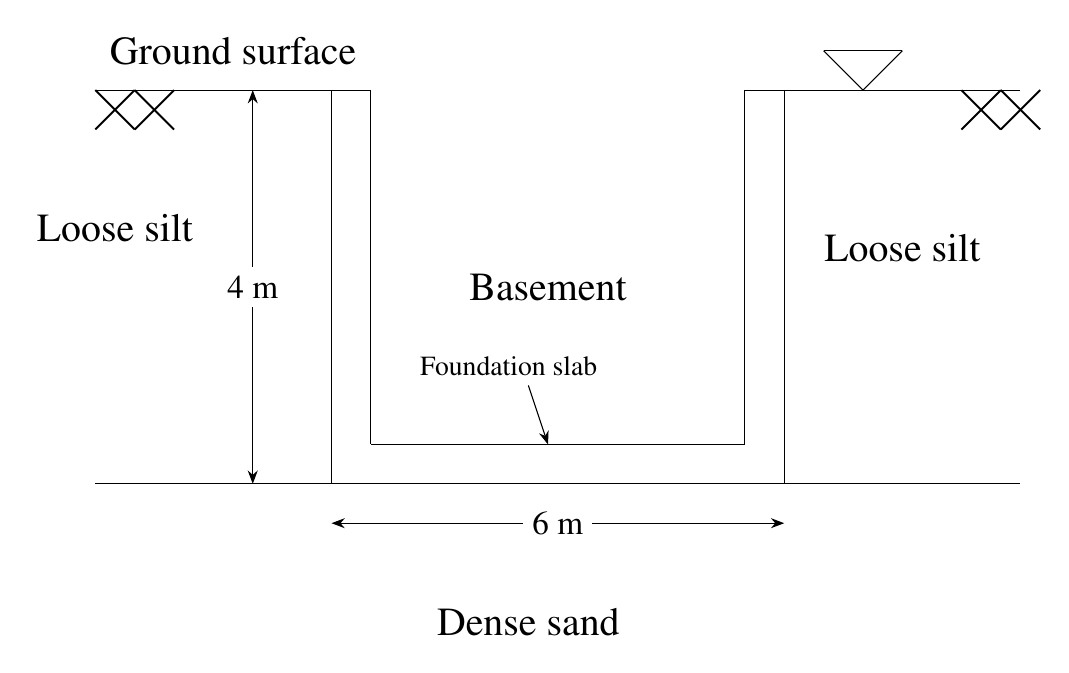
\begin{tikzpicture}
	\tikzstyle{every node}=[font=\large]
		\draw (8,9.75) to (11.5,9.75);
		\draw (11.5,9.75) to (11.5,5.25);
		\draw (11.5,5.25) to (16.25,5.25);
		\draw (16.25,5.25) to (16.25,9.75);
		\draw (16.25,9.75) to (19.75,9.75);
		\draw (11,9.75) to (11,4.75);
		\draw (11,4.75) to (16.75,4.75);
		\draw (16.75,4.75) to (16.75,9.75);
		\draw (8,4.75) to (19.75,4.75);
		\draw [<->, >=Stealth] (10,9.75) -- (10,4.75)node[pos=0.5, fill=white]{4 m};
		\draw [<->, >=Stealth] (11,4.25) -- (16.75,4.25)node[pos=0.5, fill=white]{6 m};
		\draw [->, >=Stealth] (13.5,6) -- (13.75,5.25);
		\node [font=\normalsize] at (13.25,6.25) {Foundation slab};
		\node [font=\Large] at (13.75,7.25) {Basement};
		\node [font=\Large] at (9.75,10.25) {Ground surface};
		\node [font=\Large] at (18.25,7.75) {Loose silt};
		\draw (17.25,10.25) to (17.75,9.75);
		\draw (17.75,9.75) to (18.25,10.25);
		\draw (18.25,10.25) to (17.25,10.25);
		\draw [ line width=0.7pt](19,9.75) to (19.5,9.25);
		\draw [ line width=0.7pt](19.5,9.75) to (19,9.25);
		\draw [ line width=0.7pt](19.5,9.75) to (20,9.25);
		\draw [ line width=0.7pt](19.5,9.25) to (20,9.75);
		\draw [ line width=0.7pt](8,9.75) to (8.5,9.25);
		\draw [ line width=0.7pt](8,9.25) to (8.5,9.75);
		\draw [ line width=0.7pt](8.5,9.75) to (9,9.25);
		\draw [ line width=0.7pt](8.5,9.25) to (9,9.75);
		\node [font=\Large] at (8.25,8) {Loose silt};
		\node [font=\Large] at (13.5,3) {Dense sand};
	\end{tikzpicture}
	\end{center}

	\begin{enumerate}
		\item $610$
		\item $320$
		\item $983$
		\item $693$
	\end{enumerate}

\end{enumerate}
\end{document}
